\documentclass[12pt]{article}

% Use packages %
\usepackage{graphicx, courier, amsmath, amssymb, amscd, amsfonts, mathtools, bm, esint, leftidx, extarrows, latexsym, relsize, color, tikz, comment, stmaryrd, float}
\usepackage[obeyspaces]{url}% http://ctan.org/pkg/url

% Set length %
\setlength{\textwidth}{160mm}
\setlength{\textheight}{235mm}
\setlength{\oddsidemargin}{-0mm}
\setlength{\topmargin}{-10mm}

% Define h-bar %
\newsavebox{\myhbar}
\savebox{\myhbar}{$\hbar$}
\renewcommand*{\hbar}{\mathalpha{\usebox{\myhbar}}}

% Chinese input %
%\usepackage{xeCJK} 
%\setCJKmainfont{微軟正黑體}
%\usepackage[T1]{fontenc}
%\makeatletter

% Equation number %
%\@addtoreset{equation}{section} 
%\renewcommand\theequation{{\thesection}.{\arabic{equation}}}
%\makeatletter 

% Helper Command %
\newcommand{\argmin}{\operatornamewithlimits{argmin}}
\newcommand{\rmnum}[1]{\romannumeral #1} 
\newcommand{\Rmnum}[1]{\expandafter\@slowromancap\romannumeral #1@}
\newcommand{\overbar}[1]{\mkern 1.5mu\overline{\mkern-1.5mu#1\mkern-1.5mu}\mkern 1.5mu}
\makeatother
\newcommand*{\QEDA}{\hfill\ensuremath{\blacksquare}}
\newcommand*{\QEDB}{\hfill\ensuremath{\square}}
\newcommand*{\BmVert}{\bigm\vert}
\newcommand{\bigslant}[2]{{\raisebox{.2em}{$#1$}\left/\raisebox{-.2em}{$#2$}\right.}}
\newcommand{\Nelements}[3]{\left\{ #1, ~ #2, \ldots, ~ #3 \right\}}
\newcommand{\CBrackets}[1]{\left\{#1\right\}}
\newcommand{\SBrackets}[1]{\left[#1\right]}
\newcommand{\BooBrackets}[1]{\left\llbracket#1\right\rrbracket}
\newcommand{\ParTh}[1]{\left(#1\right)}
\newcommand{\Ceil}[1]{\left\lceil#1\right\rceil}
\newcommand{\Floor}[1]{\left\lfloor#1\right\rfloor}
\newcommand{\BF}[1]{{\bf#1}}
\newcommand{\Inverse}[1]{{#1}^{-1}}
\newcommand{\Generator}[1]{\left\langle#1\right\rangle}
\newcommand{\AbsVal}[1]{\left|#1\right|}
\newcommand{\VecAbsVal}[1]{\left\|#1\right\|}
\newcommand{\BSlash}[2]{\left.#1\middle\backslash#2\right.}
\newcommand{\Divide}[2]{\left.#1\middle/#2\right.}
\newcommand{\SciNum}[2]{#1\times{10}^{#2}}
\newcommand{\Matrix}[2]{\SBrackets{\begin{array}{#1}#2\end{array}}}
\newcommand{\MatrixTwo}[4]{\ParTh{\begin{array}{cc}{#1}&{#2}\\{#3}&{#4}\end{array}}}
\newcommand{\MatrixNByN}[1]{\Matrix{cccc}{{#1}_{11} & {#1}_{12} & \cdots & {#1}_{1n} \\ {#1}_{21} & {#1}_{22} & \cdots & {#1}_{2n} \\ \vdots & \vdots & \ddots & \vdots \\ {#1}_{n1} & {#1}_{n2} & \cdots & {#1}_{nn}}}
\newcommand{\ndiv}{\hspace{-4pt}\not|\hspace{2pt}}
\newcommand{\eqdef}{\xlongequal{\text{def}}}%
\newcount\arrowcount
\newcommand\arrows[1]{\global\arrowcount#1 \ifnum\arrowcount>0
\begin{matrix}\expandafter\nextarrow\fi}
\newcommand\nextarrow[1]{\global\advance\arrowcount-1 \ifx\relax#1\relax\else \xrightarrow{#1}\fi\ifnum\arrowcount=0 \end{matrix}\else\\\expandafter\nextarrow\fi}
\newcommand{\horrule}[1]{\rule{\linewidth}{#1}}

% Tikz settings %
\usetikzlibrary{shapes,arrows}
\tikzstyle{decision} = [diamond, draw, fill=white!20, text width=4.5em, text badly centered, node distance=3cm, inner sep=0pt]
\tikzstyle{block}    = [rectangle, draw, fill=white!20, text width=8em, text centered, rounded corners, minimum height=4em]
\tikzstyle{point}    = [fill = white!20, minimum size=0.5cm]
\tikzstyle{line}     = [draw, -latex']
\tikzstyle{mapsto}   = [draw, |->]
\tikzstyle{cloud}    = [draw, ellipse,fill=red!20, node distance=3cm, minimum height=2em]

\begin{document}

\baselineskip 6.5mm
\setlength{\parindent}{0pt}
\title{ 
\normalfont \normalsize 
\horrule{0.5pt} \\[0.4cm]
\huge { \Huge Machine Learning \\ \large Answer Sheet for Homework 6 }\\
\horrule{2pt} \\ [0.5cm]
}
\author{ { \Large Da-Min HUANG } \\
{\small R04942045} \\
{\small\textit{Graduate Institute of Communication Engineering, National Taiwan University}}
}
\date{December 23, 2015}
%\allowdisplaybreaks[4]
\maketitle

\subsection*{Problem 1}

With the definition of $z_n$, rewrite the equation
\begin{align}
\min_{A,B}F\ParTh{A,B}=\dfrac{1}{N}\sum_{n=1}^{N}\ln\ParTh{1+\exp\ParTh{-y_n\ParTh{Az_n+B}}}
\end{align}
So
\begin{align}
\dfrac{\partial F}{\partial A}&=\dfrac{1}{N}\sum_{n=1}^{N}-y_n\ParTh{\dfrac{\exp\ParTh{-y_n\ParTh{Az_n+B}}}{1+\exp\ParTh{-y_n\ParTh{Az_n+B}}}}^Tz_n=\dfrac{1}{N}\sum_{n=1}^{N}-y_np^T_nz_n\\
\dfrac{\partial F}{\partial B}&=\dfrac{1}{N}\sum_{n=1}^{N}-y_n\ParTh{\dfrac{\exp\ParTh{-y_n\ParTh{Az_n+B}}}{1+\exp\ParTh{-y_n\ParTh{Az_n+B}}}}^T=\dfrac{1}{N}\sum_{n=1}^{N}-y_np^T_n
\end{align}
Hence
\begin{align}
\nabla F\ParTh{A,B}=\dfrac{1}{N}\sum_{n=1}^{N}\SBrackets{-y_nz_np_n,-y_np_n}^T
\end{align}

\QEDB

\horrule{0.5pt}

\subsection*{Problem 2}

Use the result of Problem 1 and define $\exp\ParTh{-y_n\ParTh{Az_n+B}}=\exp\ParTh{\xi_n}$, we have
\begin{align}
\dfrac{\partial^2F}{\partial A^2}&=\dfrac{\partial}{\partial A}\ParTh{\dfrac{1}{N}\sum_{n=1}^{N}-y_np^T_nz_n}\\
&=\dfrac{1}{N}\sum_{n=1}^{N}-y_n\ParTh{\dfrac{-y_n\exp\ParTh{\xi_n}\ParTh{1+\exp\ParTh{\xi_n}}z_n-y_n\ParTh{\exp\ParTh{\xi_n}}^2z_n}{\ParTh{1+\exp\ParTh{\xi_n}}^2}}z_n\\
&=\dfrac{1}{N}\sum_{n=1}^{N}-y_n\ParTh{\dfrac{-y_n\exp\ParTh{\xi_n}z_n}{\ParTh{1+\exp\ParTh{\xi_n}}^2}}z_n\\
&=\dfrac{1}{N}\sum_{n=1}^{N}\ParTh{y_n}^2\ParTh{\dfrac{\exp\ParTh{\xi_n}}{1+\exp\ParTh{\xi_n}}\ParTh{1-\dfrac{\exp\ParTh{\xi_n}}{1+\exp\ParTh{\xi_n}}}}z^2_n\\
&=\dfrac{1}{N}\sum_{n=1}^{N}z^2_np_n\ParTh{1-p_n}
\end{align}
where $y^2_n=1$ since $y_n\in\CBrackets{-1,+1}$.

The other term is
\begin{align}
\dfrac{\partial^2F}{\partial A\partial B}&=\dfrac{\partial}{\partial A}\ParTh{\dfrac{1}{N}\sum_{n=1}^{N}-y_np^T_n}=\dfrac{1}{N}\sum_{n=1}^{N}-y_n\ParTh{\dfrac{-y_n\exp\ParTh{\xi_n}z_n}{\ParTh{1+\exp\ParTh{\xi_n}}^2}}\\
&=\dfrac{1}{N}\sum_{n=1}^{N}z_np_n\ParTh{1-p_n}\\
\dfrac{\partial^2F}{\partial B\partial A}&=\dfrac{\partial}{\partial B}\ParTh{\dfrac{1}{N}\sum_{n=1}^{N}-y_np^T_nz_n}=\dfrac{1}{N}\sum_{n=1}^{N}-y_n\ParTh{\dfrac{-y_n\exp\ParTh{\xi_n}}{\ParTh{1+\exp\ParTh{\xi_n}}^2}}z_n\\
&=\dfrac{1}{N}\sum_{n=1}^{N}z_np_n\ParTh{1-p_n}\\
\dfrac{\partial^2F}{\partial B^2}&=\dfrac{\partial}{\partial B}\ParTh{\dfrac{1}{N}\sum_{n=1}^{N}-y_np^T_n}=\dfrac{1}{N}\sum_{n=1}^{N}-y_n\ParTh{\dfrac{-y_n\exp\ParTh{\xi_n}}{\ParTh{1+\exp\ParTh{\xi_n}}^2}}\\
&=\dfrac{1}{N}\sum_{n=1}^{N}p_n\ParTh{1-p_n}
\end{align}
Hence, we have
\begin{align}
H\ParTh{F}=\dfrac{1}{N}\sum_{n=1}^{N}\Matrix{cc}{z^2_np_n\ParTh{1-p_n}&z_np_n\ParTh{1-p_n}\\z_np_n\ParTh{1-p_n}&p_n\ParTh{1-p_n}}
\end{align}

\QEDB

\horrule{0.5pt}

\subsection*{Problem 3}

As $\gamma\rightarrow\infty$, we have
\begin{align}
\lim\limits_{\gamma\rightarrow\infty}\exp\ParTh{-\gamma\VecAbsVal{\BF{x}_n-\BF{x}_m}^2}=0
\end{align}
So $K$ should be a zero matrix with size $N\times N$, which is $\BF{0}_{N\times N}$.

And $\bm{\beta}$ is
\begin{align}
\bm{\beta}=\ParTh{\lambda I+K}^{-1}\BF{y}=\lambda^{-1}\BF{y}
\end{align}

\QEDB

\horrule{0.5pt}

\subsection*{Problem 4}

If $\AbsVal{y_n-\BF{w}^T\phi\ParTh{\BF{x}_n}-b}\geq\epsilon$, then
\begin{align}
\left\{
\begin{array}{ll}
\AbsVal{y_n-\BF{w}^T\phi\ParTh{\BF{x}_n}-b}-\epsilon=\xi^{\wedge}_n\text{ and }\xi^{\vee}_n=0,&\text{if }y_n-\BF{w}^T\phi\ParTh{\BF{x}_n}-b>0\\\\
\AbsVal{y_n-\BF{w}^T\phi\ParTh{\BF{x}_n}-b}-\epsilon=\xi^{\vee}_n\text{ and }\xi^{\wedge}_n=0,&\text{if }y_n-\BF{w}^T\phi\ParTh{\BF{x}_n}-b<0
\end{array}
\right.
\end{align}
 and if $\AbsVal{y_n-\BF{w}^T\phi\ParTh{\BF{x}_n}-b}<\epsilon$, then $\xi^{\wedge}_n=0$ and $\xi^{\vee}_n=0$.
Hence, we have
\begin{align}
\ParTh{\xi^\wedge_n}^2+\ParTh{\xi^\vee_n}^2=\ParTh{\max\ParTh{0,\AbsVal{y_n-\BF{w}^T\phi\ParTh{\BF{x}_n}-b}-\epsilon}}^2
\end{align}
So $P_2$ is equivalent to
\begin{align}
\min_{b,\BF{w}}\ParTh{\dfrac{1}{2}\BF{w}^T\BF{w}+C\sum_{n=1}^{N}\ParTh{\max\ParTh{0,\AbsVal{y_n-\BF{w}^T\phi\ParTh{\BF{x}_n}-b}-\epsilon}}^2}
\end{align}
with no constraints.

\QEDB

\horrule{0.5pt}

\subsection*{Problem 5}

The first term is of course
\begin{align}
\dfrac{\partial}{\partial\beta_m}\ParTh{\dfrac{1}{2}\sum_{m=1}^{N}\sum_{n=1}^{N}\beta_n\beta_mK\ParTh{\BF{x}_n,\BF{x}_m}}=\sum_{n=1}^{N}\beta_nK\ParTh{\BF{x}_n,\BF{x}_m}
\end{align}
With $\BF{w}_*$, rewrite the result of Problem 4,
\begin{align}
\text{something}&=C\sum_{n=1}^{N}\ParTh{\max\ParTh{0,\AbsVal{y_n-\sum_{m=1}^{N}\beta_mK\ParTh{\BF{x}_n,\BF{x}_m}-b}-\epsilon}}^2\\
&=C\sum_{n=1}^{N}\ParTh{\max\ParTh{0,\AbsVal{y_n-s_n}-\epsilon}}^2
\end{align}
Consider the following cases.
\begin{enumerate}
	\item $\AbsVal{y_n-s_n}\geq\epsilon$.
	
	Then we have
	\begin{align}
	\dfrac{\partial}{\partial\beta_m}\ParTh{\text{something}}&=\dfrac{\partial}{\partial\beta_m}\ParTh{C\ParTh{\AbsVal{y_n-s_n}-\epsilon}^2}\\
	&=\ParTh{2C\ParTh{\AbsVal{y_n-s_n}-\epsilon}}\dfrac{\partial}{\partial\beta_m}\AbsVal{y_n-s_n}\\
	&=-2C\ParTh{\AbsVal{y_n-s_n}-\epsilon}\text{sign}\ParTh{y_n-s_n}\dfrac{\partial s_n}{\partial\beta_m}\\
	&=-2C\ParTh{\AbsVal{y_n-s_n}-\epsilon}\text{sign}\ParTh{y_n-s_n}K\ParTh{\BF{x}_n,\BF{x}_m}
	\end{align}
	\item $\AbsVal{y_n-s_n}<\epsilon$.
	
	Then we have
	\begin{align}
	\dfrac{\partial}{\partial\beta_m}\ParTh{\text{something}}=0
	\end{align}
\end{enumerate}
So we have
\begin{align}
\dfrac{\partial F\ParTh{b,\bm{\beta}}}{\partial\beta_m}=\sum_{n=1}^{N}\beta_nK\ParTh{\BF{x}_n,\BF{x}_m}-2C\sum_{n=1}^{N}\BooBrackets{\AbsVal{y_n-s_n}\geq\epsilon}\ParTh{\AbsVal{y_n-s_n}-\epsilon}\text{sign}\ParTh{y_n-s_n}K\ParTh{\BF{x}_n,\BF{x}_m}
\end{align}

\QEDB

\horrule{0.5pt}

\subsection*{Problem 6}

First, we have
\begin{align}
e_t=\dfrac{1}{M}\sum_{m=1}^{M}\ParTh{g_t\ParTh{\tilde{\BF{x}}_m}}^2-2g_t\ParTh{\tilde{\BF{x}}_m}\tilde{y}_m+\ParTh{\tilde{y}_m}^2
\end{align}
And $e_0$ is
\begin{align}
e_0=\dfrac{1}{M}\sum_{m=1}^{M}\ParTh{0}^2-2\cdot0\cdot\tilde{y}_m+\ParTh{\tilde{y}_m}^2=\dfrac{1}{M}\sum_{m=1}^{M}\ParTh{\tilde{y}_m}^2
\end{align}
where we have used that $g_0\ParTh{\BF{x}}=0$, $\forall\BF{x}$.

So $e_t$ can be rewritten as
\begin{align}
e_t=e_0+\dfrac{1}{M}\sum_{m=1}^{M}\ParTh{g_t\ParTh{\tilde{\BF{x}}_m}}^2-2g_t\ParTh{\tilde{\BF{x}}_m}\tilde{y}_m=e_0+s_t-\dfrac{2}{M}\sum_{m=1}^{M}g_t\ParTh{\tilde{\BF{x}}_m}\tilde{y}_m
\end{align}
Hence,
\begin{align}
\sum_{m=1}^{M}g_t\ParTh{\tilde{\BF{x}}_m}\tilde{y}_m=\dfrac{M}{2}\ParTh{e_0+s_t-e_t}
\end{align}

\QEDB

\horrule{0.5pt}

\subsection*{Problem 7}

Suppose the input is $\ParTh{a,b}$ with following cases.
\begin{enumerate}
	\item $0\leq a\leq b\leq1$.
	
	Then the output should be $\ParTh{a^2,b^2}$. The line equation of these two points $\ParTh{a,a^2}$ and $\ParTh{b,b^2}$ is
\begin{align}
y=\dfrac{b^2-a^2}{b-a}\ParTh{x-a}+a^2
\end{align}
Then $\bar{g}_1\ParTh{x}$ should be
\begin{align}
\int_{0}^{1}\int_{0}^{b}\ParTh{\dfrac{b^2-a^2}{b-a}\ParTh{x-a}+a^2}dadb&=\int_{0}^{1}\left.\ParTh{\dfrac{1}{2}a^2\ParTh{x-b}+abx}\right|^{a=b}_{a=0}db\\
&=\int_{0}^{1}\ParTh{\dfrac{3}{2}b^2x-\dfrac{1}{2}b^3}db\\
&=\left.\ParTh{\dfrac{1}{2}b^3x-\dfrac{1}{8}b^4}\right|^{b=1}_{b=0}=\dfrac{1}{2}x-\dfrac{1}{8}
\end{align}

\item $0\leq b<a\leq1$.

Similarly, we have
\begin{align}
\bar{g}_2\ParTh{x}=\dfrac{1}{2}x-\dfrac{1}{8}
\end{align}
\end{enumerate}
Hence, we have
\begin{align}
\bar{g}\ParTh{x}=\bar{g}_1\ParTh{x}+\bar{g}_2\ParTh{x}=x-\dfrac{1}{4}
\end{align}
This makes sence since $\bar{g}\ParTh{x}$ and $f\ParTh{x}$ should be the same at the average value of $\SBrackets{0,1}$, which is
\begin{align}
\bar{g}\ParTh{\dfrac{1}{2}}=\dfrac{1}{2}-\dfrac{1}{4}=\dfrac{1}{4}=\ParTh{\dfrac{1}{2}}^2=f\ParTh{\dfrac{1}{2}}
\end{align}

\QEDB

\horrule{0.5pt}

\subsection*{Problem 8}

Now we have
\begin{align}
u_n\ParTh{y_n-\BF{w}^T\BF{x}_n}^2=u_ny^2_n-2u_ny_n\BF{w}^T\BF{x}_n+u_n\ParTh{\BF{w}^T\BF{x}_n}^2
\end{align}
This is equal to
\begin{align}
u_n\ParTh{y_n-\BF{w}^T\BF{x}_n}^2=\ParTh{\sqrt{u_n}y_n}^2-2\ParTh{\sqrt{u_n}y_n}\ParTh{\BF{w}^T\ParTh{\sqrt{u_n}\BF{x}_n}}+\ParTh{\BF{w}^T\ParTh{\sqrt{u_n}\BF{x}_n}}^2
\end{align}
Hence, the pseudo data is $\CBrackets{\ParTh{\tilde{\BF{x}}_n,\tilde{y}_n}}^N_{n=1}=\CBrackets{\ParTh{\sqrt{u_n}x_n,\sqrt{u_n}y_n}}^N_{n=1}$.

\QEDB

\horrule{0.5pt}

\subsection*{Problem 9}

With the rule of optimal re-weighting, we have
\begin{align}
u^{\ParTh{2}}_+=u^{\ParTh{1}}\cdot1\%,~u^{\ParTh{2}}_-=u^{\ParTh{1}}\cdot99\%\Rightarrow\dfrac{u^{\ParTh{2}}_+}{u^{\ParTh{2}}_-}=\dfrac{1}{99}
\end{align}

\QEDB

\horrule{0.5pt}

\subsection*{Problem 10}
\begin{comment}
For $L=1$, $R=6$, input vectors have 6 integers to choose in each dimension.

The different combination of $\ParTh{s,\theta}$ causes different decision stumps with $s$ has two choices $+1$ and $-1$; $\theta$ has 7 choices: $\theta\leq1$, $i<\theta\leq i+1$ and $\theta>6$, where $1\leq i\leq5$, $i\in\mathbb{N}$.
\end{comment}
Consider the following cases.
\begin{enumerate}
	\item $1<\theta\leq6$:
	
	Since $s\in\CBrackets{+1,-1}$, $d=2$ and $R-L=5$ regions to put $\theta_i$, so there are $2\times2\times5=20$ different decision stumps.
	\item $\theta\leq1$ or $\theta>6$:
	
	Then there are only $2$ decision stump: $g\ParTh{\BF{x}}=+1$ with $\ParTh{s=+1,\theta\leq1}$ or $\ParTh{s=-1,\theta>6}$; $g\ParTh{\BF{x}}=-1$ with $\ParTh{s=+1,\theta>6}$ or $\ParTh{s=-1,\theta\leq1}$ for all $\BF{x}$.
\end{enumerate}
\begin{comment}
There are $2\times7=14$ combinations, but notice that $\ParTh{s=-1,\theta>6}$ and $\ParTh{s=+1,\theta\leq1}$ lead to the same $g$, which is $g\ParTh{\BF{x}}=\ParTh{+1,+1}$, for all $\BF{x}\in\mathcal{X}$.

Also, $\ParTh{s=-1,\theta\leq1}$ and $\ParTh{s=+1,\theta>6}$ lead to the same $g$, which is $g\ParTh{\BF{x}}=\ParTh{-1,-1}$.

Let $\theta\leq1$ be the $1^{\text{st}}$ region, $i<\theta\leq i+1$ be the $\ParTh{i+1}^{\text{th}}$ region and $\theta>6$ be the $7^{\text{th}}$ region. We can find out that $\ParTh{s=+1,\theta\text{ in }j^{\text{th}}\text{ region}}$ and $\ParTh{s=-1,\theta\text{ in }k^{\text{th}}\text{ region}}$ lead to same $g$ if $j+k=8$ and $j\in\mathbb{N}$, $k\in\mathbb{N}$, $j\neq k$, due to the symmetry property. But in the $4^{\text{th}}$ region, $s=+1$ and $s=-1$ lead to different decision stumps, so there are
\end{comment}

So there are
\begin{align}
20+2=22
\end{align}
different decision stumps.

Also, this can be generalized to
\begin{align}
\underbrace{2}_{s\in\CBrackets{+1,-1}}\underbrace{d}_{\text{dimension}}{\underbrace{\ParTh{R-L}}_{\theta\text{ region}}}+\underbrace{2}_{\text{left and right region}}=2d\ParTh{R-L}+2
\end{align}

\QEDB

\horrule{0.5pt}

\subsection*{Problem 11}

First, we have
\begin{align}
K_{ds}\ParTh{\BF{x},\BF{x}^\prime}&=\sum_{i=1}^{\AbsVal{\mathcal{G}}}\ParTh{g_i\ParTh{\BF{x}}}^Tg_i\ParTh{\BF{x}^\prime}\\
&=\sum_{i=1}^{\AbsVal{\mathcal{G}}}\ParTh{s_i\text{sign}\ParTh{x_j-\theta_i}}\ParTh{s_i\text{sign}\ParTh{x^\prime_j-\theta_i}}\\
&=\sum_{i=1}^{\AbsVal{\mathcal{G}}}\text{sign}\ParTh{x_j-\theta_i}\text{sign}\ParTh{x^\prime_j-\theta_i}
\end{align}
where $\ParTh{s_i}^2=1$ since $s_i\in\CBrackets{+1,-1}$.
\begin{comment}
Now if $x_j=x^\prime_j$, we have
\begin{align}
K_{ds}\ParTh{\BF{x},\BF{x}^\prime}=\sum_{i=1}^{\AbsVal{\mathcal{G}}}\sum_{j=1}^{d}\ParTh{\text{sign}\ParTh{x_j-\theta_i}}^2=ㄅ=\sum_{i=1}^{\AbsVal{\mathcal{G}}}\sum_{j=1}^{d}1=d\AbsVal{\mathcal{G}}=2d\ParTh{R-L}+2d
\end{align}
\end{comment}

Now if $x_j=x^\prime_j$, applying the general result of Problem 11, we have
\begin{align}
K_{ds}\ParTh{\BF{x},\BF{x}^\prime}=2d\ParTh{R-L}+2
\end{align}
since all $g_i$ are the same.

If $x_j\neq x^\prime_j$, there are $\ParTh{x_j-x^\prime_j}$ different output by decision stump $g_i$ in $j^{\text{th}}$ dimension with some fixed $s_i$. One different output causes the result from $+1$ to $-1$, so the summation minus by 2 with each different output. Hence
\begin{align}
K_{ds}\ParTh{\BF{x},\BF{x}^\prime}&=2d\ParTh{R-L}+\underbrace{\ParTh{-2}}_{\text{from }+1\text{ to }-1}\times\underbrace{2}_{s\in\CBrackets{+1,-1}}\times\VecAbsVal{\BF{x}-\BF{x}^\prime}_1+2\\
&=2d\ParTh{R-L}-4\AbsVal{\BF{x}-\BF{x}^\prime}_1+2
\end{align}
where $\AbsVal{\BF{x}-\BF{x}^\prime}_1$ denotes the one-norm of $\ParTh{\BF{x}-\BF{x}^\prime}$.

\QEDB

\horrule{0.5pt}

\subsection*{Problem 12}

\begin{figure}[H]
	\centering
	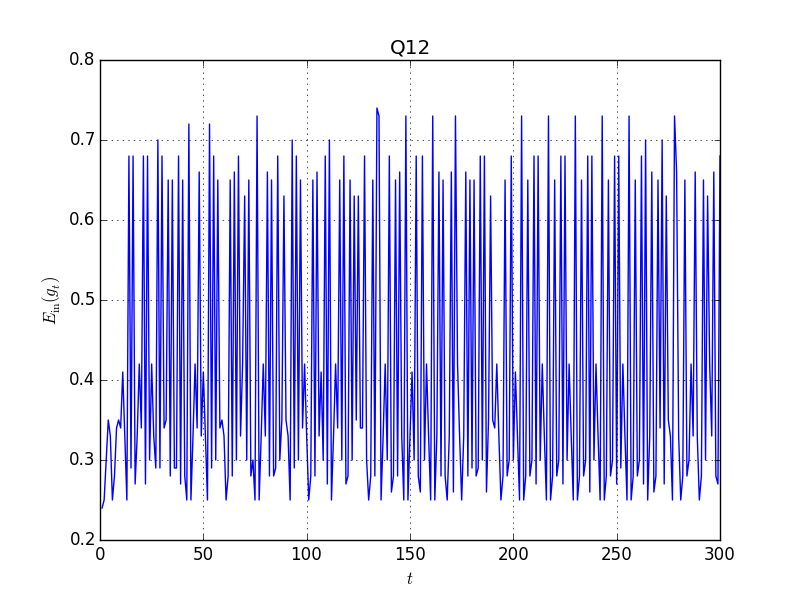
\includegraphics[scale=0.5]{Q12.png}
	\caption{Q12}
	\label{Q12}
\end{figure}
$E_{\text{in}}=0.24$, $\alpha_1=0.576339754969$.

\QEDB

\horrule{0.5pt}

\subsection*{Problem 13}

The result oscillates. Since re-weighting causes $g_{t+1}$ and $g_t$ to be very different in each iteration. So it oscillates.

\QEDB

\horrule{0.5pt}

\subsection*{Problem 14}

\begin{figure}[H]
	\centering
	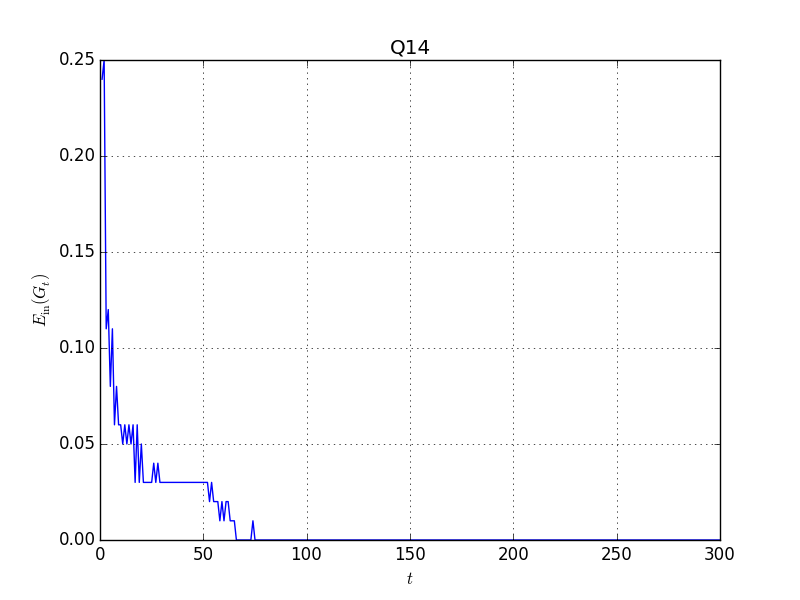
\includegraphics[scale=0.5]{Q14.png}
	\caption{Q14}
	\label{Q14}
\end{figure}
$E_{\text{in}}\ParTh{G}=0.0$.

\QEDB

\horrule{0.5pt}

\subsection*{Problem 15}

\begin{figure}[H]
	\centering
	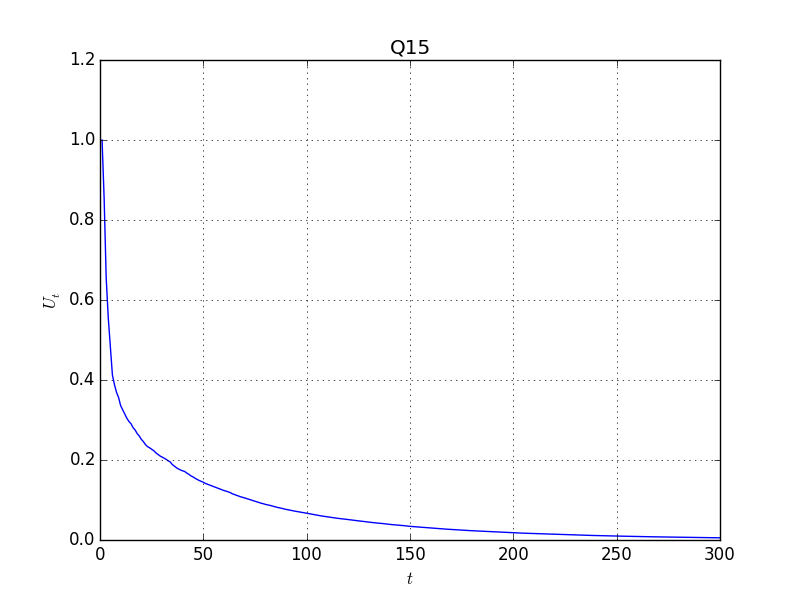
\includegraphics[scale=0.5]{Q15.png}
	\caption{Q15}
	\label{Q15}
\end{figure}
$U_2=0.8542$, $U_T=0.0055$.

\QEDB

\horrule{0.5pt}

\subsection*{Problem 16}

\begin{figure}[H]
	\centering
	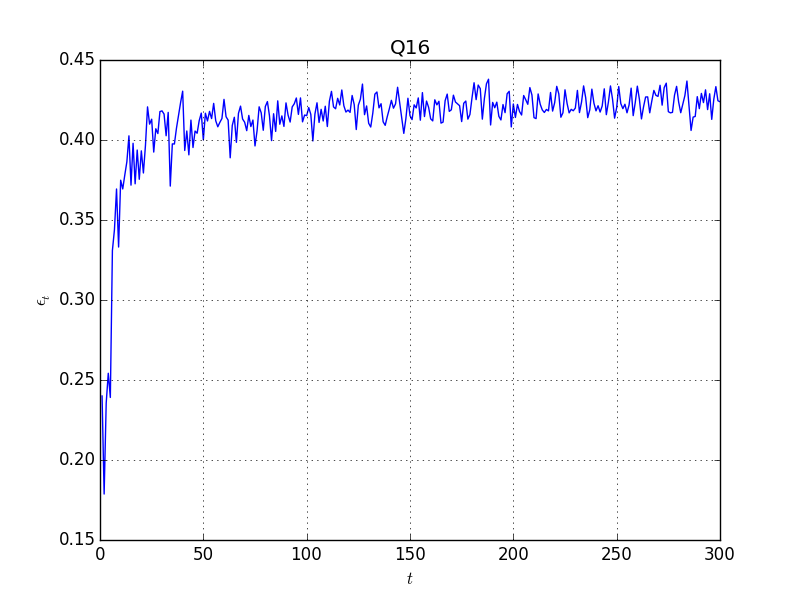
\includegraphics[scale=0.5]{Q16.png}
	\caption{Q16}
	\label{Q16}
\end{figure}
$\min\ParTh{\epsilon_t}=0.17873$.

\QEDB

\horrule{0.5pt}

\subsection*{Problem 17}

\begin{figure}[H]
	\centering
	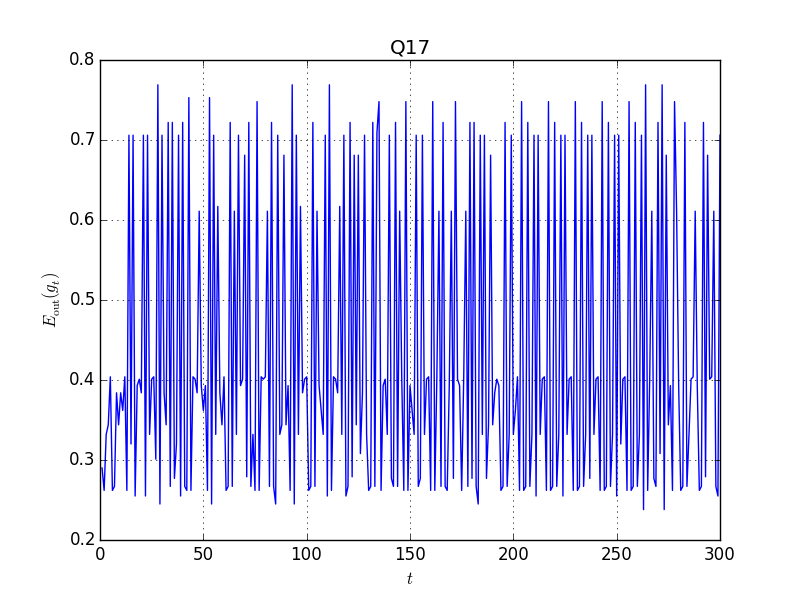
\includegraphics[scale=0.5]{Q17.png}
	\caption{Q17}
	\label{Q17}
\end{figure}
$E_{\text{out}}\ParTh{g_1}=0.29$.

\QEDB

\horrule{0.5pt}

\subsection*{Problem 18}

\begin{figure}[H]
	\centering
	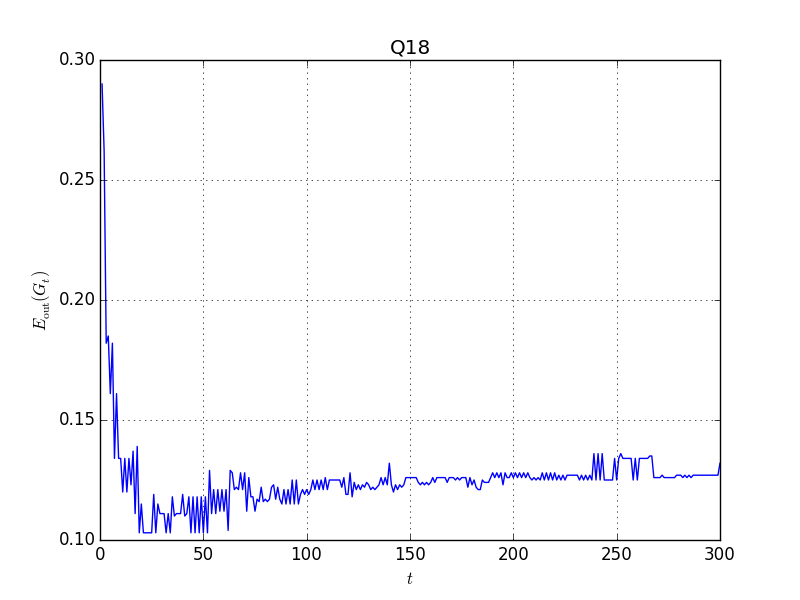
\includegraphics[scale=0.5]{Q18.png}
	\caption{Q18}
	\label{Q18}
\end{figure}
$E_{\text{out}}\ParTh{G}=0.132$.

\QEDB

\horrule{0.5pt}

\subsection*{Problem 19}

Minimum $E_{\text{in}}\ParTh{g}$ is $0.0$, with $\lambda = 0.001$, $\gamma = 32$.

\QEDB

\horrule{0.5pt}

\subsection*{Problem 20}

Minimum $E_{\text{out}}\ParTh{g}$ is $0.39$, with $\lambda = 1000$, $\gamma = 0.125$.

\QEDB

\horrule{0.5pt}

\subsection*{Problem 21}

\QEDB

\horrule{0.5pt}

\subsection*{Problem 22}

\QEDB

\horrule{0.5pt}

\section*{Reference}

\begin{enumerate}

\item[{[1]}] Lecture Notes by Hsuan-Tien LIN, Department of Computer Science and Information Engineering, National Taiwan University, Taipei 106, Taiwan.

\end{enumerate}

\end{document}